\documentclass[journal]{IEEEtran}

\usepackage{cite}
\usepackage{amsmath,amssymb}
\usepackage{graphicx}
\usepackage{booktabs}
\usepackage{url}
\usepackage[hidelinks]{hyperref}
\usepackage{multirow}

\begin{document}

\title{Multi-Scale Network Organization in\\AI-Assisted Knowledge Exploration}

\author{Alexander~Towell%
  \thanks{A.\ Towell is with the Department of Computer Science,
    Southern Illinois University Edwardsville, Edwardsville, IL 62026 USA
    (e-mail: lex@metafunctor.com).
    ORCID: 0000-0001-6443-9897.}%
}

\markboth{IEEE Transactions on Network Science and Engineering}%
{Towell: Multi-Scale Network Organization in AI-Assisted Knowledge Exploration}

\maketitle

% ============================================================
\begin{abstract}
As AI assistants become sustained intellectual partners, conversation
archives accumulate latent cognitive structure invisible in sequential
logs.  We introduce a multi-scale network analysis framework
(\emph{cognitive MRI}) and apply it to 1,908 conversations spanning 29
months.  Embedding each conversation as a vector and connecting those
exceeding a cosine similarity threshold, we analyze the resulting
network at three scales.  \textbf{Topologically}, Louvain community
detection reveals 15 knowledge communities with heterogeneous
structure: hub-and-spoke theoretical domains and tree-like applied
domains ($Q = 0.750$).  \textbf{Temporally}, monthly cumulative
snapshots show super-linear densification ($\gamma = 1.405$,
$R^2 = 0.993$) and sub-linear preferential attachment ($\beta = 0.763$),
matching growth laws of collective knowledge systems such as citation
and patent networks.  \textbf{Semantically}, LLM-extracted concepts
form a co-occurrence network with small-world topology
($\sigma \approx 6.6$), matching benchmarks for human semantic memory,
and vocabulary growth following Heaps' law
($\beta_H = 0.320$ vs.\ null $0.268$, $p < 0.001$).
These findings suggest that AI-assisted knowledge exploration produces
cognitive artifacts with deep structural regularity amenable to
principled analysis.
\end{abstract}

\begin{IEEEkeywords}
Cognitive networks, semantic similarity, knowledge graphs, densification,
small-world networks, AI-assisted learning, conversation analysis.
\end{IEEEkeywords}

% ============================================================
\section{Introduction}
\label{sec:intro}

Millions of people now conduct sustained intellectual exploration
through AI assistants.  These conversations accumulate into rich but
opaque archives: sequential logs that hide structural relationships
between topics, the dynamics of knowledge growth, and the conceptual
organization that emerges over time.

Existing work on AI conversations focuses predominantly on single-turn
quality metrics~\cite{zhao2023survey}, prompt engineering, or content
moderation.  Large-scale conversation corpora such as
WildChat~\cite{zhao2024wildchat} and
LMSYS-Chat-1M~\cite{zheng2024lmsys} have been collected and analyzed
for safety and preference, but not as cognitive artifacts with
recoverable structure.  No framework treats multi-month conversation
archives as networks amenable to the same quantitative analysis applied
to citation networks, collaboration graphs, or human semantic memory.

We address this gap with \emph{cognitive MRI}: a multi-scale network
analysis framework that transforms conversation archives into semantic
similarity networks and reveals three layers of organization:

\begin{enumerate}
\item \textbf{Topological:} Community structure distinguishing theoretical
  from applied knowledge domains, with heterogeneous internal topology
  and three distinct bridge conversation
  types~\cite{towell2025cognitive}.
\item \textbf{Temporal:} Growth laws quantitatively matching collective
  knowledge systems, including super-linear densification and sub-linear
  preferential attachment.
\item \textbf{Semantic:} A latent concept hierarchy with small-world
  topology matching human semantic memory benchmarks and sublinear
  vocabulary growth.
\end{enumerate}

The central finding is that a single individual's AI-assisted knowledge
exploration produces cognitive artifacts exhibiting structural
regularities previously observed only in large-scale collective
systems~\cite{leskovec2007graph, steyvers2005large}.  This suggests
scale-bridging organizational principles underlying both personal and
collective knowledge production.

Our approach differs from existing conversation analysis in an important
way.  While corpora like WildChat and LMSYS-Chat-1M prioritize breadth
(millions of conversations from many users), we prioritize
\emph{depth}: 1,908 conversations from a single user over 29 months.
This longitudinal single-user design enables temporal analysis
impossible with cross-sectional multi-user data, revealing how
knowledge networks grow, densify, and stabilize over time.  The
trade-off is generalizability, which we address in the discussion.

The remainder of this paper is organized as follows.
Section~\ref{sec:related} reviews related work in conversation analysis,
network science, and cognitive networks.  Section~\ref{sec:data}
describes the dataset and network construction pipeline.
Section~\ref{sec:analysis} presents the three-scale analysis.
Section~\ref{sec:discussion} discusses implications and limitations,
and Section~\ref{sec:conclusion} concludes.

% ============================================================
\section{Related Work}
\label{sec:related}

\subsection{AI conversation corpora}

Several large-scale AI conversation datasets have been released for
research.  WildChat~\cite{zhao2024wildchat} comprises one million
ChatGPT interactions collected via a browser extension, enabling studies
of user behavior, toxicity, and language distribution.
LMSYS-Chat-1M~\cite{zheng2024lmsys} provides conversations across 25
language models, focusing on model comparison and preference learning.
OpenAssistant~\cite{kopf2023openassistant} crowdsourced 161,443
messages in 35 languages for alignment research.  These corpora are
studied primarily for content analysis and model evaluation. None
applies network-theoretic methods to uncover structural relationships
between conversations or to model knowledge organization over time.

\subsection{Network science of knowledge systems}

Network science has a rich tradition of analyzing knowledge systems.
Citation networks exhibit densification
laws~\cite{leskovec2007graph}, preferential
attachment~\cite{barabasi1999emergence}, and community
structure~\cite{fortunato2010community}.  Co-authorship networks reveal
the social structure of science~\cite{newman2006modularity}, while
science-of-science models track how disciplines emerge, grow, and
interact~\cite{shi2015weaving}.  De Solla Price~\cite{price1965networks}
established that citation networks grow through cumulative advantage, a
principle later formalized as preferential attachment by Barab\'{a}si
and Albert~\cite{barabasi1999emergence}.  Leskovec et
al.~\cite{leskovec2007graph} showed that many real networks densify
over time, with edges growing super-linearly relative to nodes.

Temporal network analysis~\cite{holme2012temporal} provides frameworks
for studying how network structure evolves, including community tracking
methods that detect births, deaths, merges, and
splits~\cite{greene2010tracking, palla2007quantifying}.  These tools
have been applied extensively to social networks and collaboration
graphs but not to personal AI conversation archives, which differ from
traditional knowledge networks in being generated by a single individual
interacting with an AI system rather than by a community of researchers.

\subsection{Topic modeling and knowledge extraction}

Traditional approaches to understanding document collections include
Latent Dirichlet Allocation (LDA)~\cite{blei2003latent}, which models
documents as mixtures of topics, and neural topic models such as
BERTopic~\cite{grootendorst2022bertopic}, which use pre-trained
embeddings for topic discovery.  These methods produce flat or
hierarchical topic assignments but do not model structural relationships
between documents.

More recently, Graph RAG~\cite{edge2024graphrag} constructs entity-level
knowledge graphs from document collections to improve retrieval-augmented
generation.  While Graph RAG builds inter-document structure, it targets
information retrieval rather than cognitive analysis and does not model
temporal evolution or growth laws.  Our approach is complementary:
cognitive MRI treats conversations as atomic units connected by semantic
similarity, enabling network-level analysis of community structure,
growth dynamics, and conceptual hierarchy that topic models and
knowledge graphs do not capture.

\subsection{Cognitive network science}

Cognitive network science~\cite{siew2019cognitive} applies graph-theoretic
methods to model mental representations.  Steyvers and
Tenenbaum~\cite{steyvers2005large} demonstrated that human semantic
networks (Roget's Thesaurus, WordNet, free word association) exhibit
small-world topology with high clustering and short path lengths.
Collins and Loftus~\cite{collins1975spreading} proposed spreading
activation in semantic networks as a model of memory retrieval.
The extended mind thesis~\cite{clark1998extended} and distributed
cognition~\cite{hutchins1995cognition} argue that cognitive processes
extend beyond the brain into external artifacts, including written
records and computational tools.  Our work operationalizes this
perspective: the conversation archive functions as an externalized
cognitive workspace whose network structure reflects the user's
evolving knowledge organization.

\subsection{Comparison with existing approaches}

Table~\ref{tab:comparison} positions our framework against existing
conversation analysis methods.  Cognitive MRI is distinguished by its
combination of temporal analysis, semantic hierarchy extraction, and
network-theoretic methods applied to a longitudinal single-user archive.

\begin{table*}[t]
  \centering
  \caption{Comparison of conversation analysis approaches.  Cognitive MRI
    uniquely combines multi-month temporal analysis, semantic hierarchy
    extraction, and network-theoretic methods on a single-user archive.}
  \label{tab:comparison}
  \small
  \begin{tabular}{@{}lccccccc@{}}
    \toprule
    \textbf{Approach} &
    \textbf{Scale} &
    \textbf{Network} &
    \textbf{Temporal} &
    \textbf{Semantic} &
    \textbf{Single-user} &
    \textbf{Growth} &
    \textbf{Conversations} \\
    & & \textbf{analysis} & \textbf{dynamics} & \textbf{hierarchy} &
    \textbf{depth} & \textbf{laws} & \\
    \midrule
    WildChat~\cite{zhao2024wildchat} &
      1M users & \textemdash & \textemdash & \textemdash &
      \textemdash & \textemdash & 1,000,000 \\
    LMSYS-Chat-1M~\cite{zheng2024lmsys} &
      Multi-user & \textemdash & \textemdash & \textemdash &
      \textemdash & \textemdash & 1,000,000 \\
    OpenAssistant~\cite{kopf2023openassistant} &
      Crowdsourced & \textemdash & \textemdash & \textemdash &
      \textemdash & \textemdash & 66,497 \\
    BERTopic~\cite{grootendorst2022bertopic} &
      Varies & \textemdash & \checkmark & \textemdash &
      \textemdash & \textemdash & Varies \\
    GraphRAG~\cite{edge2024graphrag} &
      Document & \checkmark & \textemdash & \checkmark &
      \textemdash & \textemdash & N/A \\
    LDA~\cite{blei2003latent} &
      Varies & \textemdash & \textemdash & \textemdash &
      \textemdash & \textemdash & Varies \\
    \textbf{Cognitive MRI (ours)} &
      \textbf{Single user} & \checkmark & \checkmark & \checkmark &
      \checkmark & \checkmark & \textbf{1,908} \\
    \bottomrule
  \end{tabular}
\end{table*}

% ============================================================
\section{Dataset and Network Construction}
\label{sec:data}

\subsection{Dataset}

The dataset comprises 1,908 ChatGPT conversations generated by a single
user over 29 months (December 2022 to April 2025), spanning machine
learning, statistics, philosophy, programming, and cryptography.  The
archive covers five model generations: GPT-3.5 (Dec 2022--Mar 2023),
GPT-4 (Mar--Nov 2023), GPT-4 Turbo (Nov 2023--May 2024), GPT-4o
(May--Sep 2024), and reasoning models (Sep 2024--Apr 2025).  This
longitudinal span provides a natural experiment in how knowledge
networks evolve as the underlying AI capability changes.

\begin{table}[t]
  \centering
  \caption{Dataset composition by model era.  The archive spans five
    ChatGPT model generations with increasing capability.}
  \label{tab:eras}
  \small
  \begin{tabular}{@{}llrr@{}}
    \toprule
    \textbf{Era} & \textbf{Dates} & \textbf{Conv.} & \textbf{Months} \\
    \midrule
    GPT-3.5        & Dec 2022--Mar 2023 &  127 & 4 \\
    GPT-4          & Mar--Nov 2023      &  298 & 8 \\
    GPT-4 Turbo    & Nov 2023--May 2024 &  412 & 7 \\
    GPT-4o         & May--Sep 2024      &  389 & 5 \\
    Reasoning      & Sep 2024--Apr 2025 &  682 & 5 \\
    \midrule
    \textbf{Total} &                    & \textbf{1,908} & \textbf{29} \\
    \bottomrule
  \end{tabular}
\end{table}

\subsection{Embedding and weighting}

Each conversation is embedded using
nomic-embed-text~\cite{nussbaum2024nomic}, a reproducible text embedder
producing 768-dimensional L2-normalized vectors with an 8,192-token
context window.  For each conversation, user messages and AI responses
are concatenated separately.  The final embedding is a weighted average:
\begin{equation}
  \mathbf{v} = \frac{\alpha \cdot \mathbf{v}_\text{user} +
    \mathbf{v}_\text{AI}}{\|\alpha \cdot \mathbf{v}_\text{user} +
    \mathbf{v}_\text{AI}\|}
  \label{eq:embedding}
\end{equation}
where $\alpha$ controls the relative influence of user vs.\ AI content.

\subsection{Ablation study}

The weighting parameter $\alpha$ raises a methodological question:
whose content determines the semantic identity of a conversation?  User
messages reflect intent and framing, while AI responses contain detailed
explanations and generated content.  A 63-configuration ablation study
across 9 weight ratios
($\alpha \in \{100, 10, 4, 2, 1, 0.5, 0.25, 0.1, 0.01\}$) and 7
similarity thresholds
($\theta \in \{0.80, 0.825, 0.85, 0.875, 0.90, 0.925, 0.95\}$)
established that $\alpha = 2$ (user messages weighted $2{:}1$ over AI
responses) maximizes modularity at $Q = 0.750$ while preserving natural
topic structure~\cite{towell2025cognitive}.

The result is intuitive: user-heavy embeddings ($\alpha \geq 10$)
create overly fragmented communities because users phrase similar
questions in diverse ways, while AI-heavy embeddings ($\alpha \leq 0.25$)
merge distinct domains because AI responses share common explanatory
patterns.  The $2{:}1$ ratio captures the user's topical intent while
retaining enough AI content to disambiguate conversations where the user
prompt is terse but the topic is specific.

Importantly, the underlying topic distribution remains remarkably stable
across weight ratios: ML/AI content constitutes 26--37\% and general
topics 47--55\% regardless of $\alpha$, indicating that the community
structure reflects genuine thematic organization rather than weighting
artifacts.

\subsection{Threshold selection and phase transition}

Conversations are connected when their cosine similarity exceeds
$\theta$.  Table~\ref{tab:threshold} shows how network properties vary
across thresholds, revealing a phase transition at
$\theta \approx 0.875$.

\begin{table}[t]
  \centering
  \caption{Network properties across similarity thresholds.  A phase
    transition near $\theta = 0.875$ separates over-connected from
    fragmented regimes.  The chosen threshold $\theta = 0.9$ maximizes
    modularity while retaining a 75\% giant component.}
  \label{tab:threshold}
  \small
  \begin{tabular}{@{}rrrrrr@{}}
    \toprule
    $\theta$ & Nodes & Edges & GC\% & $Q$ & Comm. \\
    \midrule
    0.850 & 1,210 & 15,523 & 93.6 & 0.546 & 13 \\
    0.875 & 934 & 5,675 & 89.2 & 0.648 & 15 \\
    \textbf{0.900} & \textbf{601} & \textbf{1,718} & \textbf{75.4} &
      \textbf{0.750} & \textbf{15} \\
    0.925 & 284 & 375 & 20.8 & 0.513 & 5 \\
    \bottomrule
  \end{tabular}
\end{table}

Below $\theta = 0.875$, the network is over-connected (89--94\% giant
component, modularity below 0.65); above it, the network
catastrophically fragments ($<$21\% giant component at
$\theta = 0.925$).  The chosen threshold of $\theta = 0.9$ lies in the
post-transition regime where community structure is maximally resolved
($Q = 0.750$, 15 communities, 75.4\% giant component).  This 2.5\%
semantic distance between the over-connected and fragmented regimes
represents a narrow window separating distinct cognitive contexts.

The phase transition itself is analytically interesting: it suggests
that the semantic similarity landscape has a characteristic scale.
Conversations cluster into groups separated by approximately 10\%
cosine distance (1 $- \theta = 0.1$), with much smaller within-group
distances.  This is consistent with the existence of genuine knowledge
domains rather than a uniform continuum of topics.

% ============================================================
\section{Multi-Scale Analysis}
\label{sec:analysis}

% ------------------------------------------------------------
\subsection{Topological layer: knowledge communities}
\label{sec:topology}

\begin{figure}[t]
  \centering
  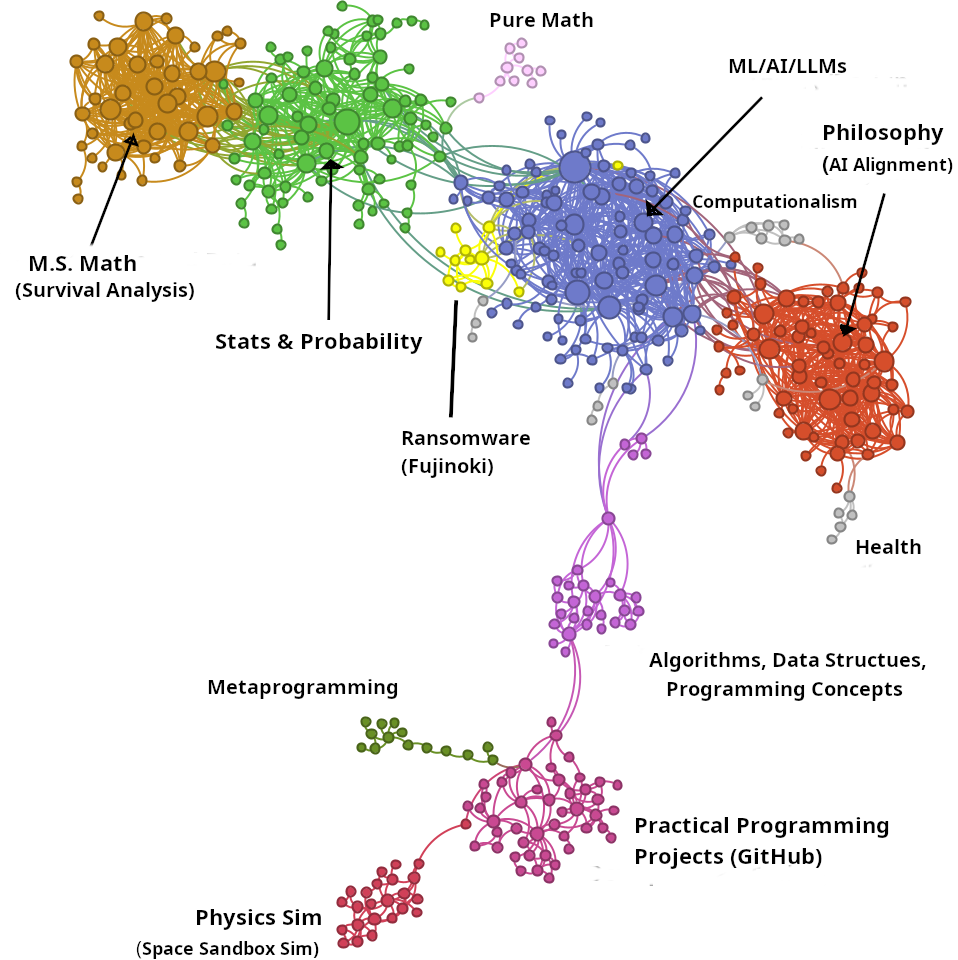
\includegraphics[width=\columnwidth]{figures/fig1-network-topology.png}
  \caption{Knowledge network at $\theta = 0.9$ showing 15 Louvain
    communities.  Theoretical domains (ML/AI, Statistics, Philosophy,
    Mathematics) form dense hub-and-spoke structures; applied domains
    (Programming, Metaprogramming) form tree-like hierarchies.  Node
    size is proportional to degree; layout by ForceAtlas2.}
  \label{fig:topology}
\end{figure}

Louvain community detection~\cite{blondel2008fast} identifies 15
communities with modularity $Q = 0.750$
(Fig.~\ref{fig:topology}).  The network exhibits heterogeneous topology
that distinguishes knowledge domain types.

\begin{table}[t]
  \centering
  \caption{Properties of the five largest communities.  Theoretical
    domains (ML/AI, Stats, Philosophy, Math) show higher clustering
    and core percentages than applied domains (Programming).}
  \label{tab:communities}
  \small
  \begin{tabular}{@{}lrrrrl@{}}
    \toprule
    \textbf{Community} & \textbf{Size} & $\bar{k}$ & \textbf{Core\%}
      & $C$ & \textbf{Type} \\
    \midrule
    ML/AI/LLM       & 103 & 8.60 & 31.1 & 0.465 & Hub-spoke \\
    Stats \& Prob.   &  82 & 7.09 & 24.4 & 0.405 & Hub-spoke \\
    Philosophy       &  65 & 10.03 & 44.6 & 0.531 & Hub-spoke \\
    M.S.\ Math       &  44 & 13.45 & 59.1 & 0.576 & Hub-spoke \\
    Programming      &  45 &  3.78 &  8.9 & 0.396 & Tree-like \\
    \bottomrule
  \end{tabular}
\end{table}

\textbf{Theoretical vs.\ applied structure.}
Table~\ref{tab:communities} summarizes the five largest communities.
Theoretical domains (ML/AI, Statistics, Philosophy, Mathematics) form
dense hub-and-spoke structures with high clustering coefficients ($C >
0.40$) and substantial core membership (24--59\%), suggesting that
theoretical knowledge organizes around central concepts with many
interconnections.  The Mathematics community is particularly dense, with
an average degree of 13.45 and 59.1\% core membership, reflecting the
tightly interconnected nature of mathematical concepts.  Applied domains
(Programming Projects, Metaprogramming) form tree-like hierarchies with
lower density ($\bar{k} = 3.78$, core only 8.9\%), reflecting the
goal-oriented, sequential nature of practical work where each project
branches from a parent concept without the dense cross-linking found in
theoretical domains.

\textbf{Core-periphery organization.}
A core-periphery decomposition~\cite{borgatti2000models} reveals that
25.6\% of nodes constitute the core (average degree 18.94), while 74.4\%
form the periphery (average degree 3.15).  Core conversations tend to
address foundational concepts that connect multiple domains, while
peripheral conversations are more specialized.

\textbf{Bridge conversations.}
Three types of bridge conversations connect otherwise distant
communities~\cite{towell2025cognitive}: \emph{evolutionary} bridges
that accumulate connections over time as the user develops
cross-domain understanding, \emph{integrative} bridges that
explicitly synthesize multiple domains in a single conversation,
and \emph{pure bridges} providing minimal but critical links between
clusters.  The highest-betweenness bridge (a conversation about
geometric mean calculations) connects four communities with
betweenness centrality of 45,468, illustrating how a single
mathematical concept can serve as a cognitive linchpin across
ML/AI, Statistics, Probability, and Tokenization.

This layer reveals \emph{what} the user knows and how knowledge domains
structurally relate.

% ------------------------------------------------------------
\subsection{Temporal layer: growth laws}
\label{sec:temporal}

\begin{figure}[t]
  \centering
  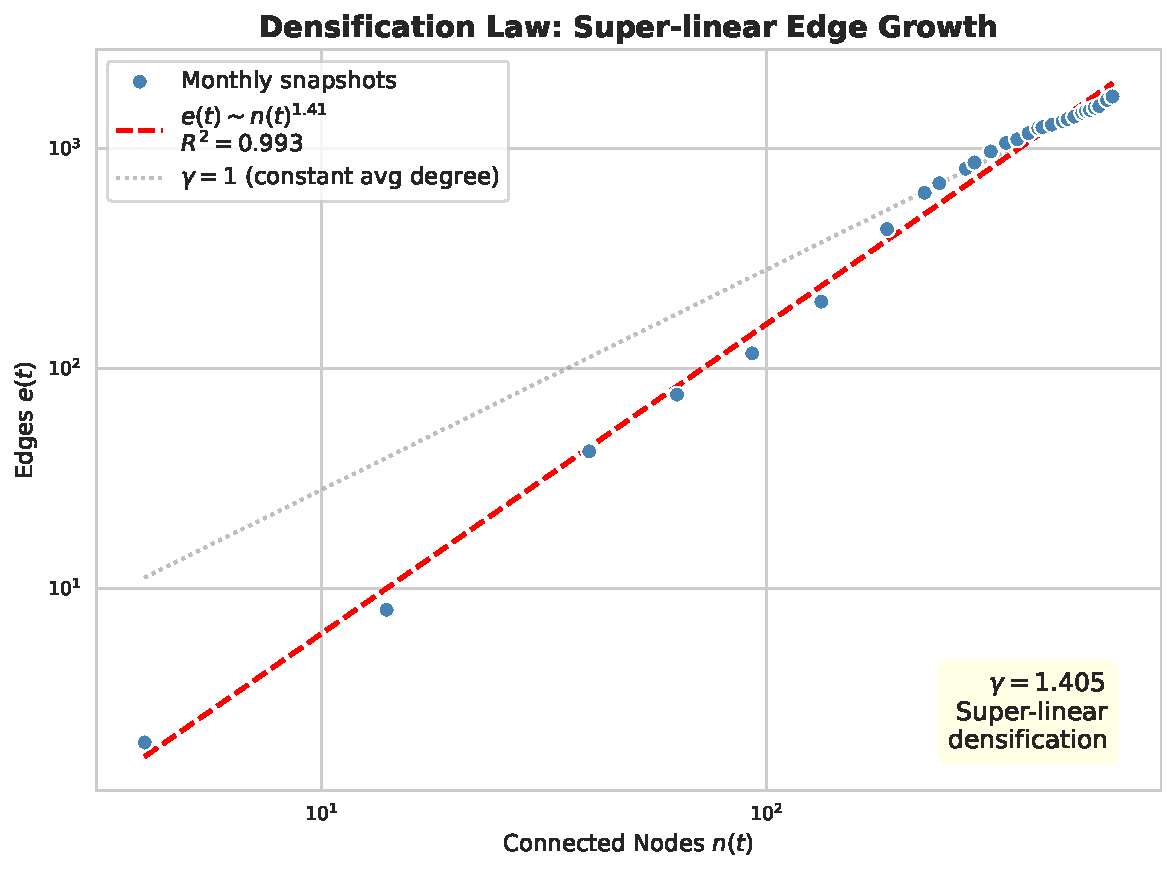
\includegraphics[width=\columnwidth]{figures/fig2-densification-law.pdf}
  \caption{Densification law: log-log plot of edges vs.\ connected nodes
    across 29 monthly snapshots.  The power-law fit
    $e(t) \propto n(t)^{1.405}$ ($R^2 = 0.993$) indicates super-linear
    densification comparable to citation and patent
    networks~\cite{leskovec2007graph}.}
  \label{fig:densification}
\end{figure}

\begin{figure}[t]
  \centering
  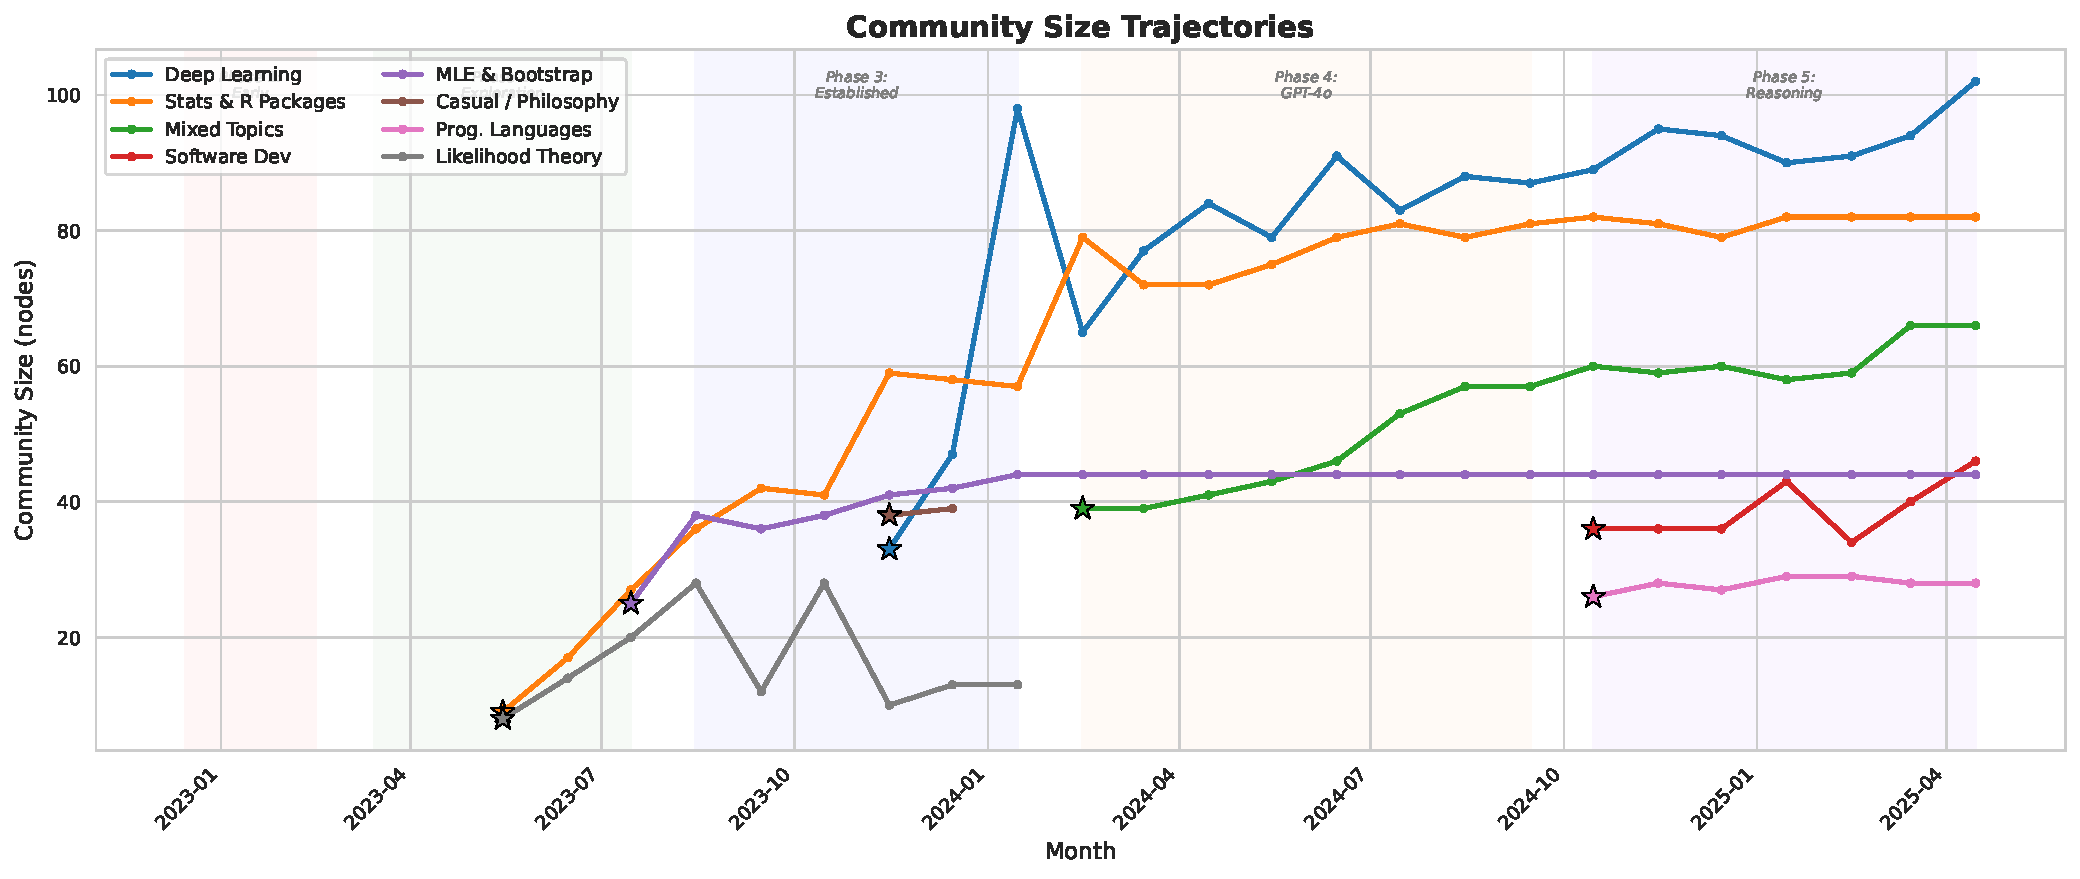
\includegraphics[width=\columnwidth]{figures/fig4-community-timeline.pdf}
  \caption{Community size trajectories over 29 months.  The two earliest
    communities (Statistics \& R Packages, Deep Learning) exhibit
    first-mover advantage, remaining the largest throughout.  Later
    communities (Software Development, Programming Languages) emerge
    during the reasoning model era.  No merge or split events occur.}
  \label{fig:timeline}
\end{figure}

\begin{figure}[t]
  \centering
  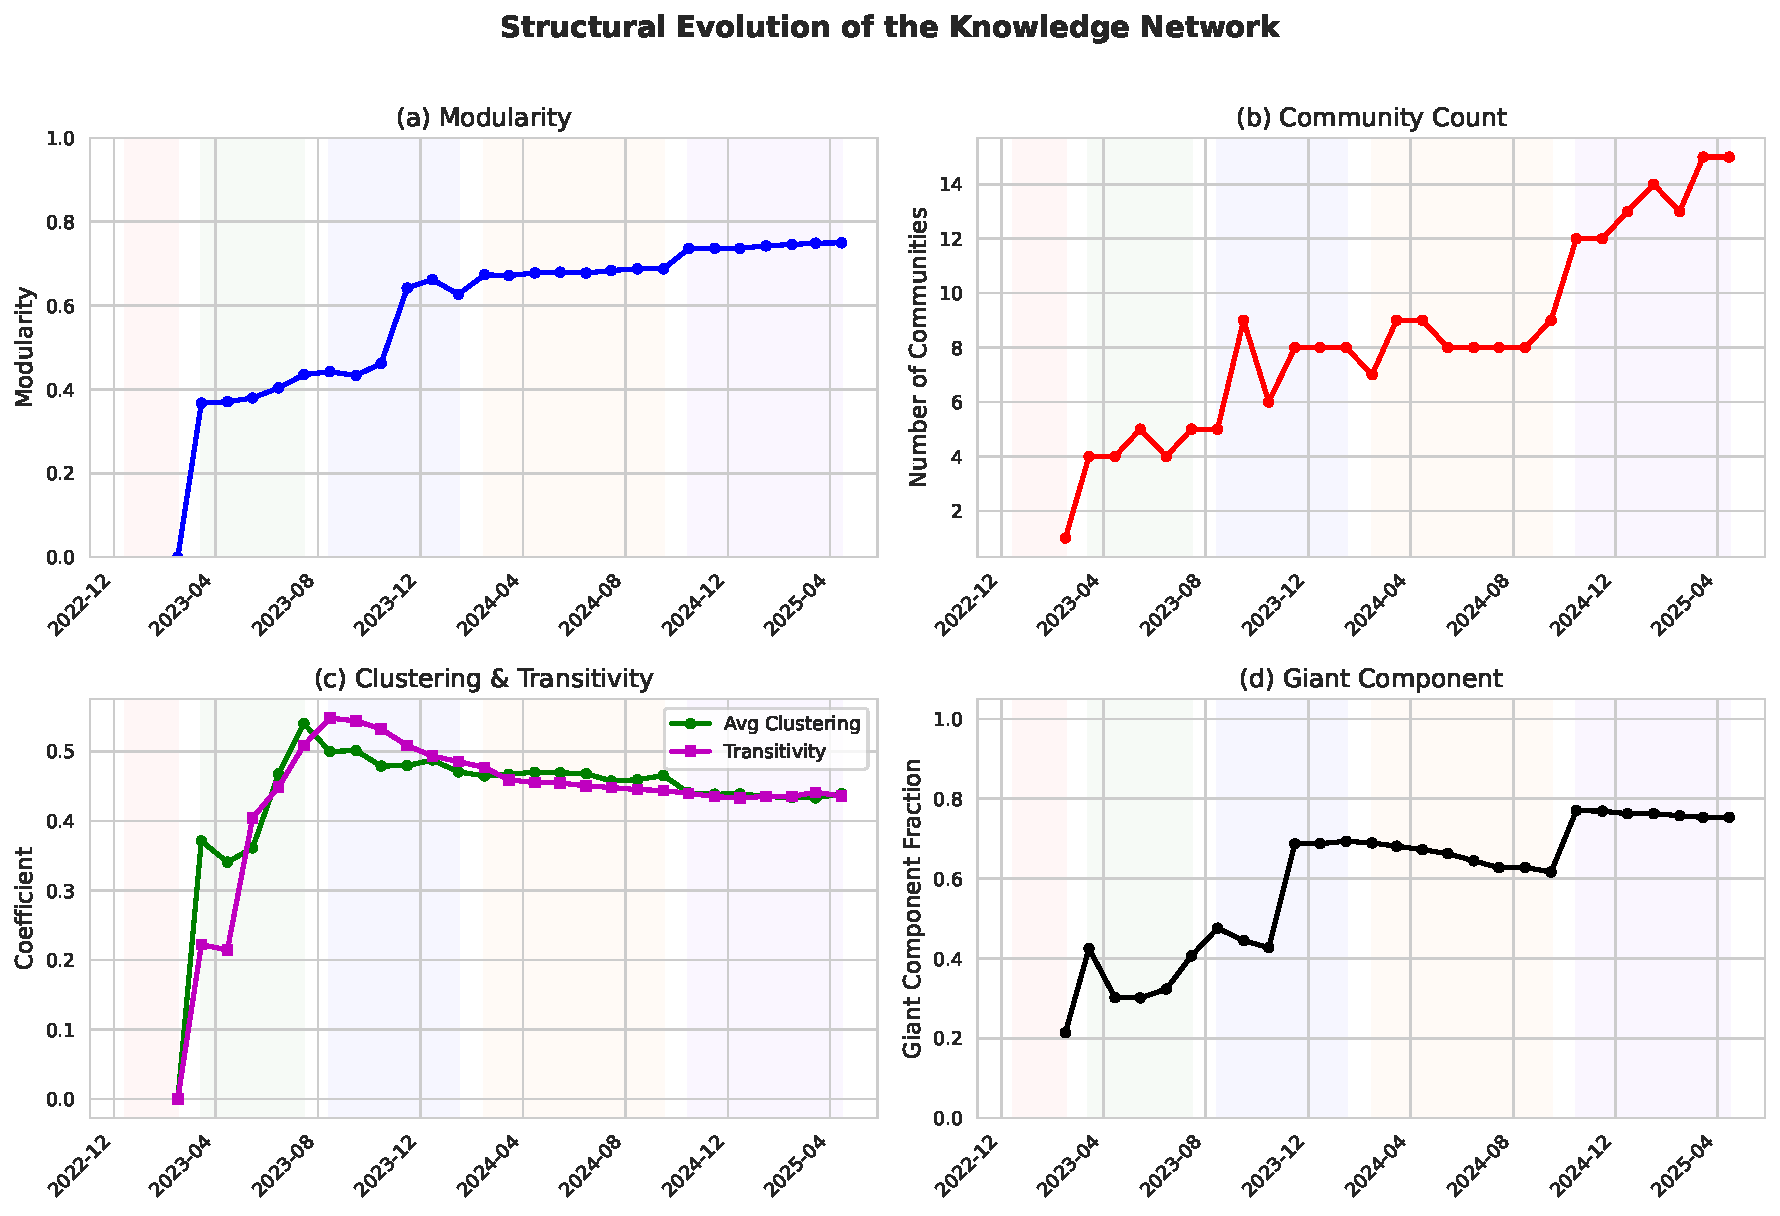
\includegraphics[width=\columnwidth]{figures/fig5-structural-evolution.pdf}
  \caption{Structural evolution over 29 months.  (a)~Modularity rises
    sharply in November 2023 and stabilizes above 0.7.
    (b)~Community count grows from 1 to 15 with distinct plateaus.
    (c)~Clustering coefficient and transitivity converge to 0.44.
    (d)~Giant component fraction stabilizes at approximately 0.75.
    Vertical dashed lines indicate model-era transitions.}
  \label{fig:evolution}
\end{figure}

Constructing 29 monthly cumulative snapshots reveals how the knowledge
network develops over time (Figs.~\ref{fig:densification}--\ref{fig:evolution}).

\textbf{Super-linear densification.}
Edges grow faster than nodes following
$e(t) \propto n(t)^{\gamma}$ with $\gamma = 1.405 \pm 0.022$
($R^2 = 0.993$, $p < 10^{-29}$; Fig.~\ref{fig:densification}).
For every doubling of connected nodes, edges increase by a factor of
$2^{1.405} \approx 2.65$.  This places the network alongside citation
networks (arXiv: $\gamma = 1.69$), patent networks ($\gamma = 1.26$),
and autonomous systems ($\gamma = 1.18$)~\cite{leskovec2007graph},
indicating that individual knowledge exploration follows the same
densification laws as collective knowledge production.
The edges-per-node ratio increases from 0.5 (January 2023) to 2.86
(April 2025), confirming that the network fills in over time as new
conversations connect to an increasingly dense existing structure.

\textbf{Sub-linear preferential attachment.}
New edges attach to existing nodes with probability
$\Pi(k) \propto k^{\beta}$ where $\beta = 0.763 \pm 0.074$
($R^2 = 0.914$), measured via the kernel estimation method
of Jeong et al.~\cite{jeong2003measuring}.  This lies between random
attachment ($\beta = 0$) and the Barab\'{a}si-Albert model
($\beta = 1$)~\cite{barabasi1999emergence}, reflecting a balanced
exploration-exploitation strategy~\cite{hills2015exploration}: popular
topics attract further exploration, but less aggressively than in
citation networks.  The sub-linearity is statistically significant,
with monthly z-scores against a random attachment null model
consistently exceeding 8.4 during the exploration phase (March--July
2023).

\textbf{Community stability.}
Modularity stabilizes at $Q > 0.6$ within 8 months and reaches 0.75 by
the final snapshot.  Tracking 40 communities across snapshots
(Fig.~\ref{fig:timeline}) reveals 189 continuations, 40 births, 25
deaths, and zero merge or split events, a pattern that contrasts
sharply with social networks where communities routinely merge and
split~\cite{palla2007quantifying}.  Knowledge domains grow internally
rather than fusing.  First-mover communities (Statistics \& R Packages,
Deep Learning) remain the largest throughout, exhibiting cumulative
advantage analogous to de Solla Price's observation in citation
networks~\cite{price1965networks}.

\textbf{Structural evolution across model eras.}
Fig.~\ref{fig:evolution} shows that key structural metrics undergo a
phase transition in November 2023, coinciding with the shift from GPT-4
to GPT-4 Turbo.  Modularity jumps from 0.45 to 0.64 in a single month,
the giant component fraction stabilizes, and the clustering coefficient
converges to its final value of 0.44.  This suggests that the network
achieves structural maturity relatively early: after approximately 8
months and 400 conversations, the large-scale organization is
established and subsequent growth fills in existing structure rather
than reorganizing it.

The five model eras (Table~\ref{tab:eras}) contribute unevenly to
network growth.  The Reasoning era (Sep 2024--Apr 2025) accounts for
36\% of all conversations (682 of 1,908) but produces proportionally
fewer new communities, consistent with the pattern of internal growth
rather than structural reorganization.  Conversations from the GPT-3.5
era, despite being the smallest cohort (127 conversations), include
several high-betweenness bridges, suggesting that early exploratory
conversations play an outsized structural role.

This layer reveals \emph{how} knowledge grows, and that individual
development follows the same quantitative laws as collective systems.

% ------------------------------------------------------------
\subsection{Semantic layer: concept hierarchy}
\label{sec:semantic}

\begin{figure}[t]
  \centering
  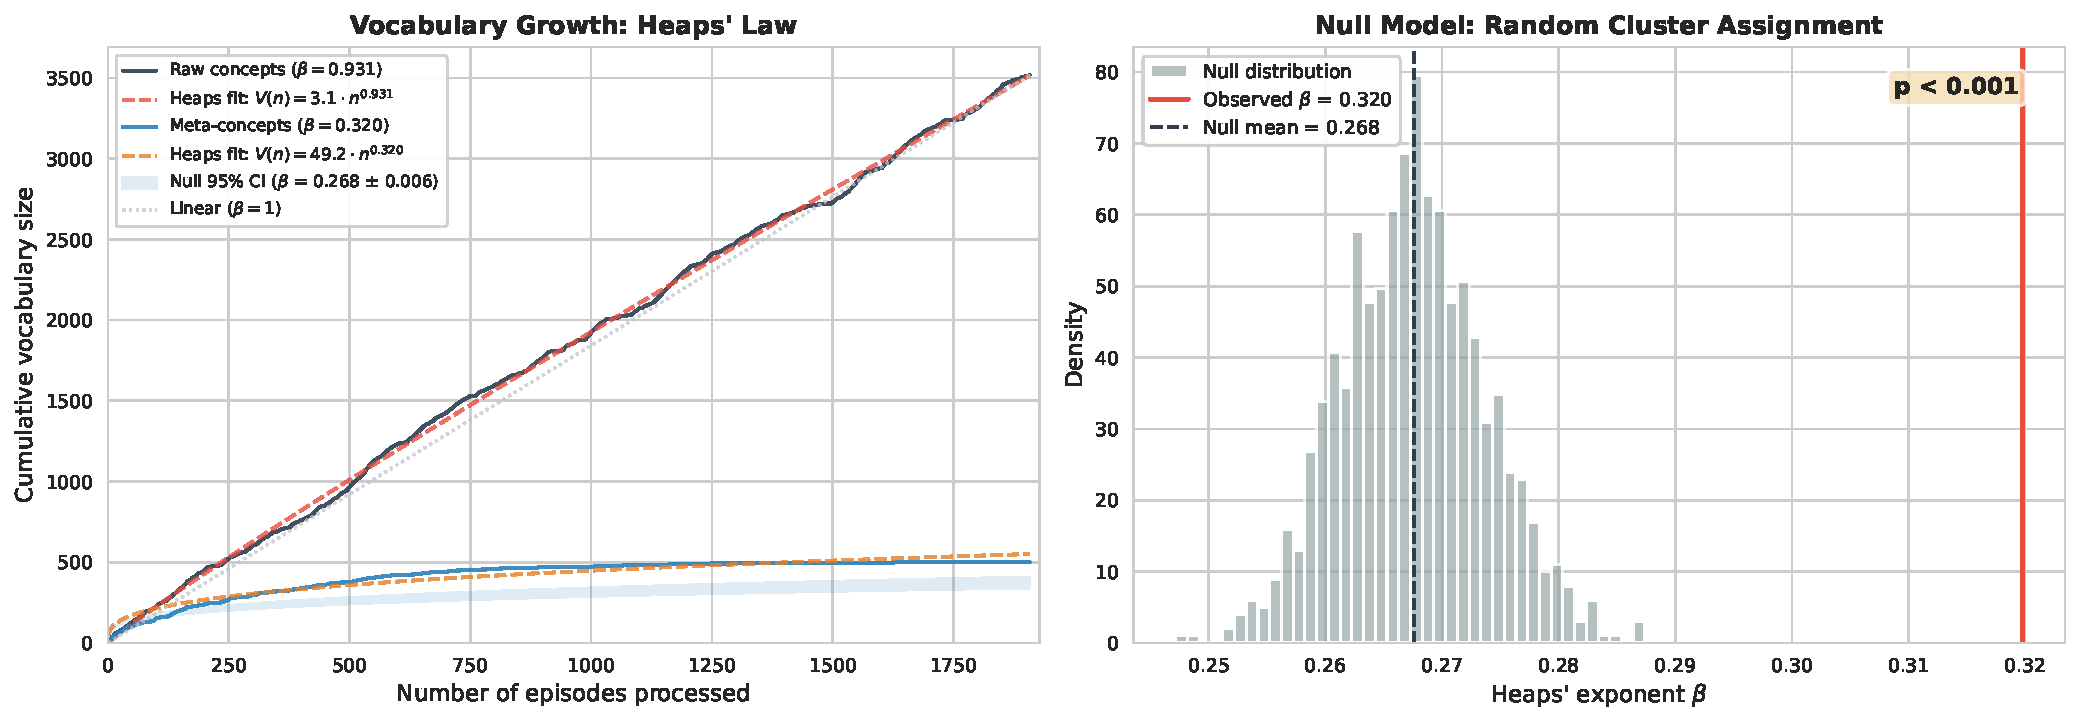
\includegraphics[width=\columnwidth]{figures/fig3-heaps-law.pdf}
  \caption{Vocabulary growth of meta-concepts follows Heaps' law
    ($\beta_H = 0.320$), significantly exceeding the random clustering
    baseline ($\beta_\text{null} = 0.268$, $p < 0.001$).
    Left: cumulative growth curve with 95\% null model band.
    Right: null distribution showing observed $\beta_H$ above all
    random permutations.}
  \label{fig:heaps}
\end{figure}

Moving beyond topological and temporal structure, we analyze the
\emph{conceptual content} of conversations using LLM-based concept
extraction, connecting to the cognitive network science tradition of
modeling mental representations as graphs~\cite{siew2019cognitive}.

\textbf{Concept extraction pipeline.}
An LLM extracts 3--10 noun-phrase concepts per conversation (mean 3.96),
yielding 6,275 raw concepts of which 3,517 are unique.  Hierarchical
clustering~\cite{ward1963hierarchical} on concept embeddings produces a
four-level hierarchy: 500 meta-concepts (agglomerative clustering with
Ward linkage), 50 themes, and 8 knowledge domains (Software Engineering
30.5\%, Mathematics \& Optimization 18\%, Statistics 14.5\%, Philosophy
\& AI Theory 13.9\%, ML \& Networks 7.8\%, DevOps 7.8\%, AI Safety
5\%, LLM Engineering 2.4\%).  A bipartite episode-concept network
(1,908 episodes, 500 meta-concepts, 7,153 edges) captures the
many-to-many relationship between conversations and concepts.

\textbf{Small-world topology.}
The concept co-occurrence network (499 nodes, 5,935 edges) exhibits
small-world structure with $\sigma \approx 6.6$, computed against 100
Erd\H{o}s-R\'{e}nyi random graphs~\cite{humphries2008network}:
clustering is $6.89\times$ higher than random graphs ($C = 0.329$
vs.\ $C_\text{rand} \approx 0.048$) while path length is only
$1.05\times$ longer ($L = 2.37$ vs.\ $L_\text{rand} \approx 2.25$).
This is comparable to benchmarks for human semantic memory networks:
Roget's Thesaurus ($\sigma \approx 13$), WordNet ($\sigma \approx 15$),
and free word association norms
($\sigma \approx 5.6$)~\cite{steyvers2005large, watts1998collective,
dedeyne2019small}.  The result is robust across clustering granularities
($k = 100$--$1{,}000$), with $\sigma > 1$ throughout.

\textbf{Sublinear vocabulary growth.}
Meta-concept vocabulary follows Heaps' law~\cite{heaps1978information}
with $\beta_H = 0.320$, significantly above a random clustering baseline
($\beta_\text{null} = 0.268$, $p < 0.001$; Fig.~\ref{fig:heaps}).
Raw concept vocabulary grows nearly linearly ($\beta = 0.931$),
confirming that the sublinear growth is a property of the semantic
clustering rather than the raw data.  Semantically coherent clusters
create meaningful distinctions: new episodes require genuinely novel
intellectual territory rather than recombining existing concepts.

\textbf{Multi-domain integration.}
77\% of conversations span two or more knowledge domains, with 35\%
spanning three or more.  Concept flow between domains is asymmetric:
Software Engineering concepts appear in 40\% of non-SE episodes
(highest broadcast reach), while ML \& Networks shows the highest
porosity at 30\% foreign concepts, consistent with its role as a
methodological bridge domain.  Size-normalized flow analysis reveals
that domains are more semantically isolated than random ($\text{mean
observed/expected} = 0.61$), but specific pairs show elevated
cross-pollination: LLM Engineering concepts appear in ML \& Networks
episodes at $2.67\times$ the expected rate.

\textbf{Orthogonality of topological and semantic structure.}
An important question is whether the concept-based domain structure
merely recapitulates the topological communities found in
Section~\ref{sec:topology}.  Normalized mutual information (NMI)
between the 8 concept domains and the 15 Louvain communities is
$\text{NMI} = 0.26$, indicating that these two decompositions capture
substantially different aspects of the knowledge network.  Topological
communities are defined by pairwise conversation similarity (who links
to whom), while concept domains are defined by shared intellectual
content (what ideas recur together).  The low NMI confirms that the
semantic layer provides genuinely new information beyond what topology
alone reveals: two conversations may share concepts without being
topologically proximate, and vice versa.

\begin{table}[t]
  \centering
  \caption{Multi-scale organization summary with literature comparisons.}
  \label{tab:summary}
  \small
  \begin{tabular}{@{}p{1.2cm}p{2.1cm}p{1.7cm}p{2.1cm}@{}}
    \toprule
    \textbf{Scale} & \textbf{Key finding} & \textbf{Metric} &
    \textbf{Literature} \\
    \midrule
    Topological &
      15 communities; hub-spoke (theory) vs.\ tree-like (applied) &
      $Q = 0.750$; core 25.6\% &
      Collab.\ networks \\
    Temporal &
      Super-linear densification; sub-linear PA &
      $\gamma = 1.405$; $\beta_\text{PA} = 0.763$ &
      arXiv $\gamma{=}1.69$, Patents $\gamma{=}1.26$ \\
    Semantic &
      Small-world concepts; Heaps' law; 77\% multi-domain &
      $\sigma \approx 6.6$; $\beta_H = 0.320$ &
      Roget's $\sigma{\approx}13$, WordNet $\sigma{\approx}15$ \\
    \bottomrule
  \end{tabular}
\end{table}

This layer reveals \emph{what concepts} organize knowledge and how they
compose across domains.  Table~\ref{tab:summary} synthesizes the three
scales with literature comparisons.

% ============================================================
\section{Discussion}
\label{sec:discussion}

\subsection{Cross-scale convergence}

The three layers are not independent views but reveal a single organizing
principle: AI-assisted exploration produces cognitive artifacts with
structural regularities previously observed only in large-scale
collective systems.  A single individual's 29 months of AI conversation
produces community structure comparable to scientific collaboration
networks~\cite{newman2006modularity, fortunato2010community}, growth
dynamics matching citation and patent
networks~\cite{leskovec2007graph}, and semantic topology matching human
semantic memory~\cite{steyvers2005large}.

This convergence across scales suggests that the mechanisms driving
knowledge organization may be scale-invariant: the same forces that
shape how scientific communities collectively structure knowledge also
shape how an individual organizes personal intellectual exploration.
The sub-linear preferential attachment ($\beta = 0.763$) is
particularly revealing: it indicates a balanced
exploration-exploitation strategy where the user revisits established
topics but maintains sufficient novelty-seeking to generate new
communities.  This balance, quantified through network growth dynamics,
provides a formal measure of intellectual exploration
style~\cite{hills2015exploration, march1991exploration}.

\subsection{Theoretical implications}

The extended mind thesis~\cite{clark1998extended} and distributed
cognition~\cite{hutchins1995cognition} argue that cognitive processes
extend into external artifacts.  Our results provide quantitative
evidence: the conversation archive functions as an externalized cognitive
workspace whose network structure mirrors properties of internal
semantic memory (small-world topology, sublinear vocabulary growth).
This suggests that AI-assisted exploration does not merely retrieve
information but actively co-constructs a structured knowledge
representation whose organization follows universal principles.

The zero merge/split pattern in community evolution is notable.
Unlike social networks where groups routinely merge and
split~\cite{palla2007quantifying}, knowledge domains grow internally.
This may reflect a fundamental difference between social and epistemic
networks: knowledge domains have clearer boundaries defined by
methodology and subject matter, whereas social groups are defined by
fluid interpersonal connections.

\subsection{The role of AI capability}

The dataset spans five model generations with substantially different
capabilities (Table~\ref{tab:eras}).  Two observations suggest that
network structure is driven primarily by the user's cognitive
organization rather than by model properties.  First, the densification
exponent $\gamma = 1.405$ fits all 29 monthly snapshots with
$R^2 = 0.993$, showing no discontinuity at model transitions.  If model
capability were driving network structure, we would expect the growth
law to change when, for example, GPT-4's improved reasoning altered the
nature of conversations.  Second, the community structure that
crystallizes by November 2023 (during the GPT-4 era) persists through
GPT-4o and reasoning models without reorganization.  New model
capabilities produce new conversations, but those conversations attach
to the existing community structure rather than reshaping it.

This stability is consistent with the interpretation that the network
reflects the user's knowledge organization, which changes gradually
through learning, rather than the AI's capabilities, which change
abruptly through model updates.  A formal test of this hypothesis
would require comparing networks from the same user interacting with
different models simultaneously, which is a direction for future work.

\subsection{Practical implications}

Conversation archives are underexploited as data sources.  They contain
recoverable cognitive structure applicable to several domains:
\begin{itemize}
\item \textbf{Personalized AI:} Network structure could inform
  recommendation of topics that bridge isolated knowledge communities.
\item \textbf{Learning analytics:} Growth law parameters ($\gamma$,
  $\beta$) provide quantitative measures of learning trajectory,
  distinguishing broad explorers from deep specialists.
\item \textbf{Knowledge auditing:} Community detection reveals blind
  spots and over-represented areas in a user's knowledge landscape.
\end{itemize}
The framework is applicable to any sustained human-AI interaction corpus,
not only ChatGPT conversations.

\subsection{Limitations and future work}

This is a single-user case study ($n = 1$).  The structural regularities
may reflect individual cognitive style rather than universal laws;
multi-user replication across diverse populations is the most important
next step.  LLM-based concept extraction introduces model-dependent
bias: different extraction models may produce different hierarchies.
Embedding-based similarity conflates topical with methodological
similarity (two conversations about ``optimization'' in different
domains may be connected despite serving different intellectual
purposes).

The threshold selection at $\theta = 0.9$, while justified by the phase
transition analysis, represents a single operating point.  Future work
should explore multi-resolution analysis across thresholds, potentially
revealing fractal community structure.

Several additional directions merit investigation.  First, causal
analysis of whether network structure predicts learning outcomes: do
users with higher densification exponents learn more effectively, or
does a particular balance of exploration and exploitation correlate with
knowledge retention?  Second, real-time cognitive MRI as a feedback
tool for AI-assisted learning, where a user could visualize their
evolving knowledge network and receive recommendations for
under-explored domains.  Third, extension to multi-user collaborative
archives, where network analysis may reveal collective knowledge
dynamics in educational settings, research groups, or organizational
knowledge management.

\subsection{Reproducibility}

All analysis code, embedding pipeline, and network construction scripts
are available via the research compendium associated with the conference
publication~\cite{towell2025cognitive}.  The conversation archive itself
cannot be shared due to privacy considerations (it contains personal
intellectual content), but the methodology is applicable to any
conversation export in JSON format.  The embedding model
(nomic-embed-text) is open-source and deterministic given fixed inputs,
ensuring reproducibility of the network construction step.

% ============================================================
\section{Conclusion}
\label{sec:conclusion}

We presented cognitive MRI, a multi-scale network analysis framework for
AI conversation archives that reveals structure at three complementary
scales.  Applied to 1,908 conversations spanning 29 months and five
model generations, the framework yields the following principal results:

\begin{enumerate}
\item \textbf{Topological structure:} 15 knowledge communities with
  modularity $Q = 0.750$, exhibiting heterogeneous topology (hub-spoke
  for theoretical domains, tree-like for applied domains) and a
  core-periphery organization where 25.6\% of conversations form
  a densely connected core.
\item \textbf{Temporal growth laws:} Super-linear densification
  ($\gamma = 1.405$, $R^2 = 0.993$) and sub-linear preferential
  attachment ($\beta = 0.763$), placing the network alongside citation
  and patent networks in the landscape of real-world growth dynamics.
\item \textbf{Semantic hierarchy:} A four-level concept hierarchy
  (500 meta-concepts, 50 themes, 8 domains) with small-world topology
  ($\sigma \approx 6.6$) comparable to human semantic memory benchmarks,
  and vocabulary growth following Heaps' law ($\beta_H = 0.320$,
  $p < 0.001$ above random baseline).
\end{enumerate}

The central finding is that individual-scale AI-assisted knowledge
exploration exhibits quantitatively similar structural laws to
collective knowledge systems.  This convergence across scales, combined
with the stability of network structure across model generations,
suggests that the organizational principles reflect properties of human
knowledge production rather than artifacts of any particular AI system.
As AI-assisted exploration becomes ubiquitous, frameworks like cognitive
MRI provide principled tools for understanding the cognitive structures
that emerge from this new form of intellectual partnership.

% ============================================================
\section*{Acknowledgment}

AI tools were used for concept extraction during the semantic analysis
phase.  \LaTeX{} formatting assistance was provided by an AI coding
assistant.  All intellectual contributions, analysis design,
interpretation, and writing are the author's own.

% ============================================================
\bibliographystyle{IEEEtran}
\bibliography{refs}

\end{document}
